%\documentclass[sigplan,review,nonacm,10pt]{acmart}
\documentclass[sigplan,nonacm,10pt]{acmart}

\usepackage{minted}
\usepackage{makecell}
\usepackage{booktabs}
\usepackage{microtype}
\graphicspath{ {./figs/} }
\newcommand\aste{%
$^{(\ast)}$
}
\usepackage[subtle]{savetrees}

% https://tex.stackexchange.com/questions/655620/how-to-make-acmart-stop-complaining-about-missing-country-in-affiliation
\makeatletter
\def\@ACM@checkaffil{% Only warnings
    \if@ACM@instpresent\else
    \ClassWarningNoLine{\@classname}{No institution present for an affiliation}%
    \fi
    \if@ACM@citypresent\else
    \ClassWarningNoLine{\@classname}{No city present for an affiliation}%
    \fi
    \if@ACM@countrypresent\else
        \ClassWarningNoLine{\@classname}{No country present for an affiliation}%
    \fi
}
\makeatother

%%
%% \BibTeX command to typeset BibTeX logo in the docs
\AtBeginDocument{%
  \providecommand\BibTeX{{%
    Bib\TeX}}}

%% Rights management information.  This information is sent to you
%% when you complete the rights form.  These commands have SAMPLE
%% values in them; it is your responsibility as an author to replace
%% the commands and values with those provided to you when you
%% complete the rights form.
\setcopyright{acmcopyright}
\copyrightyear{2023}
\acmYear{2023}
%\acmDOI{XXXXXXX.XXXXXXX}

%% These commands are for a PROCEEDINGS abstract or paper.
\acmConference[CS294]{CS294}{Fall 2023}{Berkeley, CA}
%%
%%  Uncomment \acmBooktitle if the title of the proceedings is different
%%  from ``Proceedings of ...''!
%%
%%\acmBooktitle{Woodstock '18: ACM Symposium on Neural Gaze Detection,
%%  June 03--05, 2018, Woodstock, NY}
%\acmPrice{15.00}
%\acmISBN{978-1-4503-XXXX-X/18/06}


%%
%% Submission ID.
%% Use this when submitting an article to a sponsored event. You'll
%% receive a unique submission ID from the organizers
%% of the event, and this ID should be used as the parameter to this command.
%%\acmSubmissionID{123-A56-BU3}

%%
%% For managing citations, it is recommended to use bibliography
%% files in BibTeX format.
%%
%% You can then either use BibTeX with the ACM-Reference-Format style,
%% or BibLaTeX with the acmnumeric or acmauthoryear sytles, that include
%% support for advanced citation of software artefact from the
%% biblatex-software package, also separately available on CTAN.
%%
%% Look at the sample-*-biblatex.tex files for templates showcasing
%% the biblatex styles.
%%

%%
%% The majority of ACM publications use numbered citations and
%% references.  The command \citestyle{authoryear} switches to the
%% "author year" style.
%%
%% If you are preparing content for an event
%% sponsored by ACM SIGGRAPH, you must use the "author year" style of
%% citations and references.
%% Uncommenting
%% the next command will enable that style.
%%\citestyle{acmauthoryear}
\settopmatter{printacmref=false}

%%
%% end of the preamble, start of the body of the document source.
\begin{document}

%%
%% The "title" command has an optional parameter,
%% allowing the author to define a "short title" to be used in page headers.
% \title{TidalSim: Mixing Functional Simulation, $\mu$Arch Models, and RTL Simulation for Rapid Microarchitectural Iteration and Evaluation}
\title{TidalSim: Multi-Level Simulation for Rapid Microarchitectural Iteration and Evaluation}

%%
%% The "author" command and its associated commands are used to define
%% the authors and their affiliations.
%% Of note is the shared affiliation of the first two authors, and the
%% "authornote" and "authornotemark" commands
%% used to denote shared contribution to the research.

\author{\href{https://orcid.org/0000-0001-6934-6577}{Vighnesh Iyer}, Raghav Gupta, Dhruv Vaish, Young-Jin Park, Charles Hong, Sophia Shao, \href{https://orcid.org/0000-0003-2324-1715}{Borivoje Nikolić}}
\email{{vighnesh.iyer,rgupta,dvaish,bora}@berkeley.edu}
\affiliation{%
  \institution{UC Berkeley}
}

% \author{Borivoje Nikolić}
% \email{bora@eecs.berkeley.edu}
% \orcid{0000-0003-2324-1715}
% \affiliation{%
%   \institution{UC Berkeley}
% }


%%
%% By default, the full list of authors will be used in the page
%% headers. Often, this list is too long, and will overlap
%% other information printed in the page headers. This command allows
%% the author to define a more concise list
%% of authors' names for this purpose.
\renewcommand{\shortauthors}{Iyer, Vighnesh et al.}

\begin{abstract}

% Due to the end of Moore's law and Dennard scaling...
% lol no

Existing approaches to microarchitecture simulation cannot simultaneouly deliver the three goals of high throughput, low latency, and high fidelity.
Rapid RTL-level microarchitectural iteration and evaluation on real applications is enabled by a simulator that can meet these three objectives.
Our multi-level simulator combines functional ISA-level simulation, microarchitectural warmup models, and RTL simulation to produce accurate IPC traces.
This new paradigm of multi-level simulation opens the door to an efficient and accurate DSE methodology, rapid evaluation of RTL-level optimizations, and automatic extraction of RTL-level traces of interesting and unique segments of long workloads.

\end{abstract}

% \received{20 February 2007}
% \received[revised]{12 March 2009}
% \received[accepted]{5 June 2009}

\maketitle

\section{Introduction}

% Fill only the first page
% 1. Describe the problem
%   use an example to introduce the problem, consider this scenario..., how would you evaluate it?
% 2. State your contributions
%   write as a bulleted list, make the contributions refutable, make them specific
%   each claim that we make should contain a forward reference to a section that provides evidence for that claim

% What is the typical microarchitectural design and iteration process?
Designing a microprocessor involves evaluating a proposed microarchitecture on representative workloads, and optimizing the microarchitecture to meet the power, performance, and area targets for a set of applications based on your target market.
Evaluation of a microarchitecture is typically a lengthy process and these long evaluation cycles bottleneck the iteration loop of making a microarchitectural change and seeing its impact.
The agile design of microprocessors demands an evaluation methodology with low latency that enables rapid microarchitectural development, optimization, and tuning.

\subsection{The Problem}

% What workloads do we use to evaluate our decisions?
Consider this scenario: you (a microarchitect) are designing a next-generation microprocessor for a mobile SoC optimized for web browsing, and you want to make changes to improve the PPA of your design.
Microarchitects rarely start completely from scratch; instead, you have the RTL from the previous generation's microprocessor, a functional ISA-level model, and perhaps a performance model.
Let's say you also have representative web and mobile applications and perhaps some smaller benchmark suites from the software engineering side.

The microarchitecture iteration loop involves making changes to the RTL, evaluating them for correctness and performance on the real-world applications the SoC will see, and using the evaluation results (e.g. performance metrics, identified bottlenecks, profiling traces, RTL-level waveforms) to guide further microarchitectural exploration (see Figure \ref{fig:uarch_iteration_loop}).

\begin{figure}
  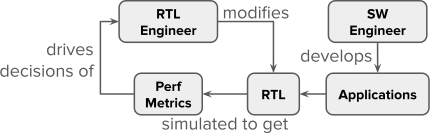
\includegraphics[width=\linewidth]{dynamic/tidalsim/uarch_iteration_flow.pdf}
  \caption{Typical microarchitecture iteration loop}
  \label{fig:uarch_iteration_loop}
\end{figure}

% Want to consider 1) evaluation of a new microarchitectural structure, 2) optimizing the uArch of a given structure, 3) tuning hardware parameters.
% What kinds of decisions do we want to make during the process?
There are broadly three categories of RTL changes you might make:
\begin{enumerate}
  % Evaluate the usefulness of the structure, what new state is needed
  \item Creating a completely new structure (e.g. a vector unit, a prefetcher, a new type of branch predictor)
  % Optimization of the uArch e.g. reordering support, multiple dispatch and parallelism
  \item Optimizing the microarchitecture of an existing structure or pipeline (e.g. reducing the dispatch latency from the ROB, adding a new forwarding path)
  % Parameter tuning and its impact on performance
  \item Parameterizing an RTL unit or tuning hardware parameters that already exist (e.g. tuning cache hierarchy and sizing, queue sizing in the LSU)
\end{enumerate}

For the latter two types of RTL changes, the bottleneck in their evaluation is often not the architectural modeling, RTL development, or verification, but rather measuring the impact of the changes on real workloads.
If you only had access to traditional simulation techniques, you would be stuck with these options:
\begin{itemize}
  \item `Fast' but low startup latency simulators (functional and architectural models) which would lead to decisions being made on likely inaccurate data
  \item `Fast' but high startup latency simulators (FPGA-based simulators) which would bottleneck the speed of microarchitectural iteration
  \item `Slow` simulators (RTL simulators) that would not be able to run a full workload to begin with in a reasonable time
\end{itemize}

You would like the best of all worlds: a simulator that is fast (high throughput to run real workloads), has low startup latency (to get performance results from a proposed change quickly), and is accurate (so you can make microarchitectural decisions confidently).

% I want this table to show up on the second page!
\begin{figure*}[!hbt]
  \small
  % Alladin (analytical models, often specialized for kernel accelerators), functional ISA simulation, gem5-style perf sim (this is the most diverse category), RTL sim, FPGA prototype (high fidelity if IO modeling isn't an issue), FPGA emulator (Firesim), Emulation (Palladium)
  \begin{tabular}{>{\raggedright\arraybackslash}p{2.5cm}>{\raggedright\arraybackslash}p{2cm}>{\raggedright\arraybackslash}p{2cm}>{\raggedright\arraybackslash}p{2cm}>{\raggedright\arraybackslash}p{2.5cm}>{\raggedright\arraybackslash}p{3cm}>{\raggedright\arraybackslash}p{2cm}}\toprule
  \textbf{Simulator Type} & \textbf{Examples} & \textbf{Throughput} & \textbf{Latency} & \textbf{Accuracy} & \textbf{Metrics} & \textbf{Cost} \\\midrule
  Analytical Models & Alladdin, Accelergy & ??? & seconds & ??? & Execution time + PPA estimates & Minimal \\
  \midrule
  Functional ISA-Level Simulators & spike, dromajo, qemu & 100-1000 MIPS & $<1$ second & Zero & Dynamic instruction count + mix & Minimal \\
  \midrule
  Trace-Based and Cycle-Level Simulators & gem5, Sniper, ZSim, SST, MARSSx86 & 100 KIPS - 10 MIPS & $<1$ minute & $\approx10-50\%$ IPC error & uArch metric (IPC, MPKI) traces & Minimal \\
  \midrule
  RTL Simulators & Verilator, VCS, Xcelium & 10 KIPS & 2-10 minutes & Cycle-exact & RTL-level traces and uArch metrics & Minimal \\
  \midrule
  FPGA Prototypes & HAPS, Protium & $\approx$50 MIPS & 2-6 hours & Cycle-exact, but IOs not timing accurate & Visibility of subset of RTL signals & \$10k+ \\
  \midrule
  FPGA-Based Emulators & Firesim & $\approx$10 MIPS & 2-6 hours & Cycle-exact & RTL-level traces and uArch metrics & \$10k+ \\
  \midrule
  ASIC-Based Emulators & ZeBu, Palladium & $\approx$10 MIPS & < 1 hour & Cycle-exact & RTL-level traces and uArch metrics & \$10M+ \\
  \midrule
  Multi-Level Simulation & TidalSim \textbf{(this paper)} & $\approx$10 MIPS & minutes & < 5\% IPC error & RTL-level traces and uArch metrics & Minimal \\
  \bottomrule
  \end{tabular}
  \caption{The spectrum of analytical, architectural, and microarchitectural simulation techniques and how they compare on various axes. Numbers assume simulation of a low core count SoC.}
  \label{fig:spectrum_of_simulators}
\end{figure*}

\subsection{Our Contributions}

In this paper, we propose a simulation methodology that dramatically reduces the evaluation time overhead of microarchitectural iteration.
We demonstrate:

\begin{itemize}
  \item A technique to combine functional ISA-level simulation, microarchitectural warmup models, and RTL-level simulation to produce a `multi-level' simulator capable of running at 10 MIPS with low startup latency and high accuracy (under 5\% IPC error with respect to full RTL simulation)
  \item The ability to produce detailed IPC traces (with time-granularity of 10k instruction windows) for long running workloads (millions of dynamic instructions) in a matter of seconds
\end{itemize}

\section{Background}

% Later: I should say that all these tasks involve benchmark extraction and rapid evaluation and I can help in all of these tasks with tidalsim
% However, for this paper, I will focus on just the simulation and performance estimation aspect
There are many tasks involved in the design of a microprocessor such as architectural and performance modeling, the RTL design itself, verification, power and area estimation, and of course performance evaluation.
In this paper, we only focus on improving the latency and accuracy of performance evaluation.
The primary means of performance evaluation is simulation, so we will first survey existing simulation techniques.

% I want this table to show up on the 3rd page!
\begin{figure*}[!hbt]
  \small
  \begin{tabular}{>{\raggedright\arraybackslash}p{2cm}>{\raggedright\arraybackslash}p{2cm}>{\raggedright\arraybackslash}p{2cm}>{\raggedright\arraybackslash}p{2cm}>{\raggedright\arraybackslash}p{2cm}>{\raggedright\arraybackslash}p{2cm}>{\raggedright\arraybackslash}p{2cm}}\toprule
  \textbf{Sampling Technique} & \textbf{Interval Length} & \textbf{\# of Intervals Simulated} & \textbf{Interval Selection} & \textbf{Functional Warmup} & \textbf{Detailed Warmup} & \textbf{Time Granularity} \\\midrule
  Simpoint & 1-100M & 50-100 & BBV + k-means & Optional & $\approx$0.1-1M & Interval length \\
  \midrule
  SMARTs & 100k-1M & $\approx$10k & Reservoir sampling & Required & $\approx$10k & Entire workload \\
  \midrule
  TidalSim \textbf{(this paper)} & 10k & 10-100 & BBV + k-means & Required & $\approx$2k & Interval length \\
  \bottomrule
  \end{tabular}
  \caption{Comparison between the two classes of sampled simulation methodologies.}
  \label{fig:sampled_simulation}
\end{figure*}

\subsection{The Spectrum of Simulation Techniques}

There are many analytical, architectural, and microarchitectural simulation techniques that have been developed over the past few decades spanning the gamut on various axes:

\begin{itemize}
  \item \textbf{Throughput}: how many instructions can be simulated per real second? Often given in MIPS (Millions of Instructions Per Second).
  \item \textbf{Accuracy}: how accurate are the output metrics of the simulator with respect to the modeled SoC in its real environment?
  \begin{itemize}
    % Early stage vs late stage / exploratory vs tuning: some simulators are designed for exploring the impact of very high-level parameters while others are for refinement
    \item This axis is correlated to whether a simulator is designed for early-stage exploration of high-level parameters or for late-stage tuning of a refined microarchitecture.
  \end{itemize}
  \item \textbf{Startup latency}: how long does it take from the moment the simulator's parameters or inputs are modified to when the simulator begins executing the first simulated instruction?
  \item \textbf{Metric diversity}: the types of metrics that the simulator can output. This is closely related with the simulator's use-case (for early vs late stage design).
  % TODO: we can actually compute a $ per million insts metric (considering both initial capital cost + per instruction cost AND the cost if cloud by-the-hour services are available)
  \item \textbf{Cost}: what hardware platform does the simulator run on and how much does it cost to run a simulation? In this paper, we don't precisely compute this metric.
\end{itemize}

% Talk about simulation methodologies + their limitations
The range of existing simulation techniques are summarized in Table \ref{fig:spectrum_of_simulators}.
Notably, there aren't any options for RTL-level microarchitecture iteration where we need high throughput, low startup latency, high accuracy, and low cost.
While it may seem like ASIC-based emulators are a good option if only their cost was brought down, the reality is that the cost of these systems is not merely incidental due to lack of engineering effort, but fundamental to the technology they use.

% Also how much fidelity is typical from perf sims? (cite paper on arch simulators considered harmful).
Cycle-level or trace-based simulators might be another option, however they suffer from an unfavorable tradeoff between accuracy, throughput, and flexibility\cite{arch_sim_considered_harmful, the_whole_truth}.
`Accurate' simulators, such as Sniper, are accurate since they have been `calibrated' against a real hardware datapoint: however, there is no evidence that they are accurate when their parameters are changed (as there is no silicon to compare against), and furthermore they have limited flexibility\cite{arch_sim_survey, x86_arch_sim_study}.
More general-purpose simulators, like gem5, are not as `accurate' as Sniper on a known silicon datapoint, but are much more flexible: however they suffer from low throughput.
Performance simulators suffer from unbounded errors, and it is often difficult or impossible to trace the source of errors between the simulator and the target they are intended to model\cite{diagsim}.

\subsection{Sampled Microarchitectural Simulation}

% Talk about sampled simulation and some prior work on that
Notwithstanding the accuracy and flexibility limitations of performance simulators (e.g. gem5, Sniper, ZSim), prior work has attempted to significantly improve the throughput of these simulators using \textit{sampling}.
At a high-level, sampling involves simulating most of the workload on a fast functional simulator, and only playing parts of the simulation on a more detailed performance (cycle-level or trace-based) simulator.
This way, the simulation can run at nearly the speed of a functional simulator (10s-100s of MIPS), while still being able to estimate performance.

Sampling works, by first, splitting a workload's execution trace into intervals of a particular number of dynamic instructions.
Then, only specific intervals (samples) are actually run in performance simulation.
Depending on the sampling technique there may be a need for functional warmup (injecting an estimated state of long-lived microarchitectural components such as caches and branch predictors).
There is also a detailed warmup period during which short-lived microarchitectural states (e.g. ROB, LSU, pipeline) are warmed up by executing the interval, before performance metrics collection begins.

\begin{figure}
  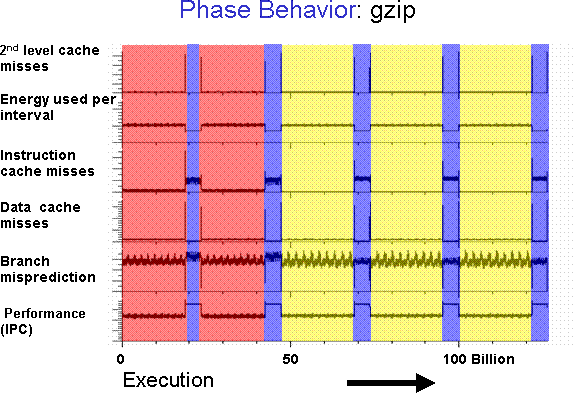
\includegraphics[width=\linewidth]{multi-level-sim/simpoint-gzip_phases.png}
  \caption{Program phases in gzip discovered using Simpoint-style interval embedding and clustering\cite{simpoint3}.}
  \label{fig:simpoint}
\end{figure}

% Sampled simulation adds error on top of the existing modeling error in performance simulators.
There are broadly two types of sampling proposed in the literature: Simpoint-style sampling\cite{simpoint3} and SMARTs-style sampling\cite{smarts} (summarized in Figure \ref{fig:sampled_simulation}).

\subsubsection{Simpoint-Style Sampling}

The Simpoint technique embeds each interval with its `basic block vector' (BBV), which indicates which basic blocks of the workload were traversed in that interval.
Then, the interval embeddings are clustered using k-means clustering, and one or more representative intervals are selected per-cluster.

% Talk about phase behavior of programs
The intuition behind Simpoint's interval selection strategy is that intervals that traverse the similar basic blocks are likely to have similar microarchitectural behaviors.
Therefore, programs can be broken up into \textit{phases} that exhibit similar basic block traversal patterns and thus have similar performance metrics (see Figure \ref{fig:simpoint}).

Those intervals are run in performance simulation to extract their performance metrics and those metrics are extrapolated to produce performance metrics for the full workload trace.
Simpoint sampling usually does not require functional warmup since the interval lengths are large enough to warm up long-lived microarchitectural state.
Since we can estimate performance for each interval separately, the time-granularity of Simpoint IPC traces is the interval length.

\subsubsection{SMARTs-Style Sampling}

The SMARTs technique selects which intervals to run in performance simulation via reservoir sampling, with no knowledge of the instruction-level characteristics of the interval.
It uses far more and much shorter intervals than the Simpoint technique.
Since the intervals are short, functional warmup is required to initialize microarchitectural structures in performance simulation.

The performance metrics gathered from each interval serve as samples of the true distribution of IPC across the workload.
The SMARTs technique uses the central limit theorem to estimate the IPC for the entire workload and give statistical confidence bounds on the estimate.
Since the SMARTs technique has no understanding of the relationship of one interval to any other, it can only estimate performance metrics with the time-granularity of an entire workload.

\section{The Concept of Multi-Level Simulation}

% Introduce the problem and your idea using *examples* and only then present the general case

We can see that existing simulation techniques cannot simultaneously deliver on all the axes of high accuracy, high throughput, low startup latency, and low cost.
This bottlenecks the microarchitectural iteration loop since evaluation is either 1) too slow to run on realistic workloads, or 2) too inaccurate to make decisions, or 3) incurs too high a cost or has too long of a startup latency to use in the iteration loop.

\subsection{Issues with Existing Simulation Techniques}

% What's wrong with perf sims (low accuracy).
% What's wrong with RTL/FPGA sims (bad throughput or high latency + high cost).
% What's wrong with sampled perf sims (compounded low accuracy, not a good tradeoff).

Cycle-level or trace-based simulators suffer from low accuracy and unbounded errors which are further exacerbated by sampled simulation which \textit{adds sampling error on top of modeling error}.
RTL simulation delivers high accuracy, but with very low throughput.
FPGA or ASIC based simulators can match the accuracy of RTL simulation, but come with high startup latency and cost.

We propose TidalSim: a multi-level simulator that can deliver the accuracy of RTL simulation, with the throughput of FPGA-based simulators, and a low startup latency.

\subsection{Our Proposal}

% Sampled multi-level simulation!
To achieve high throughput we will leverage simulation sampling techniques, but instead of using architectural simulators for performance metric estimation, we will use RTL simulators.
We specifically employ a sampling methodology similar to Simpoint, but with functional warmup and shorter interval lengths.

\subsubsection{Why Use RTL Simulators?}

% Why multi-level simulation? Why not arch sim 2-level sim? Why go down to RTL?
% Why not just go into perf simulators?
% Don't want to design perf model and then design RTL to match that - what a waste, not agile!
% Aren't "trends" enough? Not when we care about small IPC changes! The absolute number matters!
% Miscorrelation vs RTL *compounds* over simulation time!
% the correlation problem gets compounded 2x - sampling error + perf sim - RTL sim correlation errors
% Also what are the special things we can get from RTL simulation that perf sim can't get us?

Existing sampled simulators mix functional simulators and architectural simulators (e.g. gem5, Sniper, SST).
We continue to use functional warmup models similar to those in architectural simulators, but we use RTL simulation for extracting performance metrics.

\paragraph{What is the benefit of introducing RTL simulators into the mix?}

For one, it has been shown that performance simulators can be wildly inaccurate\cite{arch_sim_considered_harmful, arch_sim_survey} and often have unbounded modeling errors in addition to sampling errors, while RTL simulation is cycle-accurate.
Also, using RTL simulation for performance estimation means there is no need to perform correlation between the performance simulators and RTL.

Having RTL also enables us to derive accurate PPA numbers for the SoC as a whole using a traditional synthesis flow, whereas performance simulators can at best give vague estimates.
Since our flow already leverages sampled simulation for performance trace estimation, we can apply a similar flow to extrapolate a full power trace using post-RTL power estimation CAD tools.

Finally, RTL simulators produce special collateral that cannot be produced from performance simulators, such as RTL-level waveforms and detailed microarchitectural events.
Thus, we can obtain many short waveforms that reflect unique aspects of the simulated workloads, suitable for applications ranging from power modeling to coverpoint synthesis.

\paragraph{Why was mixing RTL simulation with sampled simulation not attempted before?}

% We can't try to 'fix' perf models. And in the new open source research era we have RTL! for every part of the system too! we can draw realistic conclusions finally! cite Chipyard, ESP, OpenPiton

In order to use RTL simulation, you need to have RTL for the design point that you are trying to evaluate.
In the past, this has been difficult since the only available open-source RTL was low quality, low performance, poorly parameterizable, and not extensible.
Furthermore, to use RTL simulation with sampling requires a way to restore and resume simulation from architectural checkpoints: this can tightly couple the low-level state injection logic with a specific RTL design point.

Recently, we have seen an explosion of design frameworks with high quality open-source RTL for every part of a complete SoC\cite{chipyard, open_esp, openpiton, xiangshan, pulpv2, blackparrot}.
These design frameworks support extensive parameterization, easy integration of external RTL, and can leverage hardware compiler frameworks\cite{firrtl} to automate generation of state injection code.
It has now become possible to leverage RTL for large workload simulation and microarchitectural design space exploration.

\subsubsection{Why Use Simpoint-Style Sampling?}

% fine time-granularity, high liklihood of unique traces, eventual ability to extrapolate across workloads via binary-agnostic embedding similarity

SMARTs-style sampling only gives us a single number for a performance metric (e.g. IPC).
While it can be more accurate and have statistical error bounds, the intervals chosen for simulation are often redundant (i.e. they have similar microarchitectural characteristics).
When performing microarchitectural exploration, we often want a detailed view of IPC behaviors \textit{within} a workload's trace to, for example, diagnose pathological behaviors visible as unexpected IPC spikes.

Simpoint-style sampling uses interval embeddings and clustering, so the intervals chosen for simulation are at least guaranteed to have unique basic block traversal patterns.
This form of sampling gives us interval length time-granularity of the IPC trace.
Furthermore, if we can develop binary-agnostic interval embeddings, it will allow the simulator to extrapolate performance metrics \textit{across workloads} which have intervals with similar embeddings.

\subsection{TidalSim Overview}

\begin{figure}
  
\includegraphics[width=\linewidth]{dynamic/tidalsim/overview.pdf}
  \caption{An overview of the steps involved in the TidalSim flow.}
  \label{fig:tidalsim_overview}
\end{figure}

A high-level overview of the TidalSim flow is shown in Figure \ref{fig:tidalsim_overview}.
The steps of the flow are:

\begin{enumerate}
  \item Call a functional simulator with a workload binary to get a commit log (contains PC, decoded instruction, register operands, and memory transactions for each committed instruction)
  \item Split the commit log into intervals with a fixed number of instructions
  \item Something else
\end{enumerate}
We use a similar technique as Simpoint in performing commit log dumping from a functional simulator, 

\section{Implementation}

\subsection{Interval Embedding Strategies}

For embeddings:
Binary agnostic
Microarchitecture agnostic
- BBVs - binary aware, uarch unaware
- NPS - binary unaware, uarch unaware
- BBVs + uarch features - binary aware, uarch aware
- Ideal - binary unaware, uarch aware

\subsection{Basic Block Identification and BBV Embedding}

\subsection{Architectural Checkpointing}

\subsection{Functional Warmup Models}

\subsection{RTL Simulation}

\subsubsection{State Injection}

DMI is too slow, a total bottleneck. Also doesn't work for uArch state.
We use force/release which avoid needing a debug simulator, is very fast, and general.

\subsubsection{State Injection Caveats}

Not all state can be cleanly injected!

\subsubsection{Performance Metric Extraction}

\subsection{Extrapolation}

\section{Results}

What benchmarks?
What baseline SoC?
What is the baseline?

\subsection{Interval Clustering}

\subsection{IPC Trace Reconstruction}

\section{Future Work}

\subsection{Functional Warmup}

Add figure about general functional warmup strategies.

\subsection{Embedding-Driven Extrapolation}

\subsection{Better Interval Embeddings}

\subsection{Arch Checkpoint Reloading Validation}

\subsection{Applications}

Power, perf, 2 verif angles (coverpoint synthesis + bootstrapping fuzzing)

\subsection{Actual `Tidal'Sim}

Right now this is more like one-directional sim. ISA model -> warmup models -> RTL sim.
Works fine for shrinkwrapped examples with no interrupts (external or timer), no outside interactions.

But consider things like timer interrupts or syscall proxying to the host via tether! Or external interrupts!
The ISA-level simulation needs an understanding of time to make consistent decisions or error will compound!

Unifying embedding-based interval selection with random interval selection, increasing random sampling when errors appear to be high.

\section{Related Work}

\textbf{Sampled Simulation:} Work in this area involves techniques to select a small number of intervals from an execution trace to simulate in detail. 
\textbf{Statistical Sampling} involves the use of statistical methods on an estimated performance metric such as IPC-based reservoir sampling in SMARTS \cite{smarts}.
\textbf{Profile-based Sampling} analyzes a program/execution trace to identify representative intervals. SimPoint \cite{simpoint3} clusters per-interval basic block frequency vectors to identify intervals of interest. Tidalsim applies this technique (albeit to RISC-V traces). 
TidalSim results in lower error due to the use of RTL simulation in a multi-level setup and employs more efficient functional warmup than SMARTS.

\textbf{Functional Warmup:} Cold long-lived microarchitectural blocks such as caches and cache-like structures (TLBs and BTBs) lead to significant simulation error. Strategies to quickly warm them include continuous simulation of module behavior as seen in SMARTS \cite{wunderlich2003smarts}, reduced-length module simulation using estimates of memory access reuse latencies as seen in MRRL \cite{haskins2003memory} and BRRL \cite{eeckhout2005blrl}, and functional checkpoint and restore of module contents as seen in MTR \cite{barr2005accelerating}. TidalSim currently employs. MTR for its low temporal overhead, accuracy, and simplicity. 
Similar techniques have been proposed for branch predictors in MRRL and BHM \cite{kluyskens2007branch} (reduced length simulation) and branch trace compression \cite{barr2006branch}.

\textbf{Multi-level Simulation:} LiveSim \cite{hassani2016livesim} uses emulation for statistical sampling (SMARTS) and architectural state checkpointing followed by detailed simulation with microarchitecture models. However, it suffers from microarchitecture model correlation error, unlike TidalSim which uses cycle-exact RTL simulation. 

\section{Conclusion}

% Add Github links to all forks and tidalsim top

\begin{acks}
Acks go here (Seah, Joonho, Sophia, Chris)
\end{acks}

\bibliographystyle{ACM-Reference-Format}
\bibliography{references}

% \appendix

\end{document}
\endinput
